%=========================================================================
% fig-tuning-vectorization-pooling.tex
%=========================================================================

\begin{figure}[t]

  \centering
  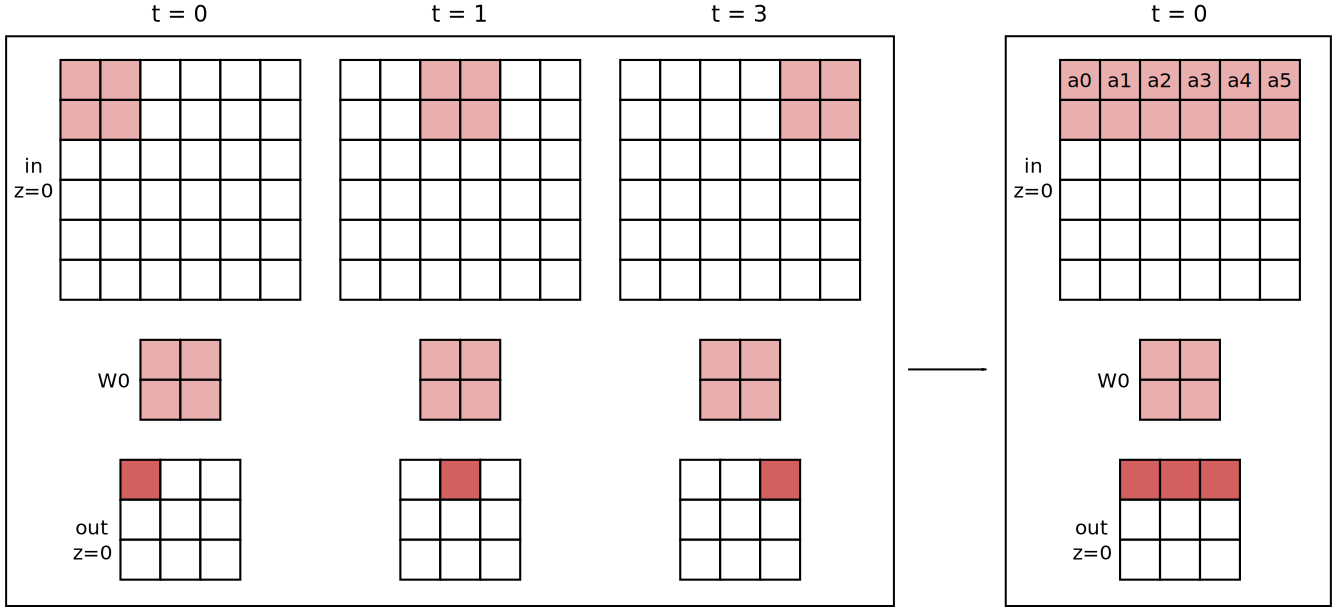
\includegraphics[width=0.9\tw]{fig-tune-vector-pooling.svg.pdf}

  \caption{\textbf{Vectorization Strategy for Pooling Layer --} A 6x6x1
    input is downsampled using a 2x2x1 filter to produce a 3x3x1 slice of
    the output. The box on the left illustrates the scalarized approach
    that takes three computational timesteps to calculate the first row
    of the output. The box on the right illustrates the vectorized
    approach that takes a single computational timestep to perform the
    same computations.}

  \label{fig-tuning-vectorization-pooling}

\end{figure}
